\newpage
\section{Input \& Output}

\begin{figure}[h!]
	\centering
	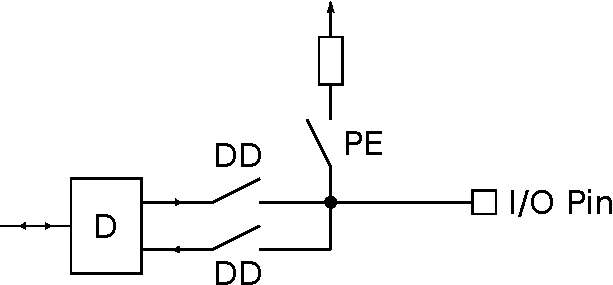
\includegraphics[scale=1]{../fig/io.pdf}
	\caption{Vereinfachtes I/O Blockschaltbild}
\end{figure}

\subsection{I/O Register}

\begin{table}[h!]
	\centering
	\begin{tabular}{l l l}
	Kürzel & Name & Beschreibung \\
	\hline
	PTxD
		& Data Register	
		& enthält die I/O Zustände \\
	PTxDD
		& Data Direction
		& gibt die Funktion an (INPUT oder OUTPUT) \\
	PTxPE
		& Pullup Enable
		& interner Pullup (EIN oder AUS) \\
	PTxSE
		& Output Slewrate
		& Schnell oder langsam schalten (en = 30ns, $\overline{en}$ = 3ns) \\
	PTxDS
		& Drive Strength
		& Stombelastbarkeit (en = 10mA, $\overline{en}$ = 2mA)
	\end{tabular}
	\caption{Übersicht der elementaren I/O Register 
		\protect \cite[S.163]{hcs08}}
\end{table}

\subsection{I/O Initialisiren}

\subsubsection{Eingang}
\begin{lstlisting}
PTADD = PTADD & 0xFE;	// set direction of pin PTA0 as input
input = PTAD & 0x01;	// read the state of pin PTA0;
\end{lstlisting}

\subsubsection{Ausgang}
\begin{lstlisting}
PTADD = PTADD | 0x01;	// set direction of pin PTA0 as output

PTAD = PTAD & 0xFE;	// set the pin PTA0 to low
PTAD = PTAD | 0x01;	// set the pin PTA0 to high
\end{lstlisting}

\newpage
\subsection{Beispiele}

\subsubsection{LED ein- \& ausschalten auf MC-Car mit Assembler}
\lstinputlisting[firstline=59 , lastline=80]{../src/blink_asm/Sources/main.asm}

\subsubsection{LED ein- \& ausschalten auf MC-Car mit C}
\lstinputlisting[firstline=19, lastline=47]{../src/blink_c/Sources/main.c}
